\documentclass[a4paper, 11pt]{article} % 11 pt font
\usepackage[utf8]{inputenc}
\usepackage[american]{babel}
\usepackage[margin=1in]{geometry} % 1 in margins
\usepackage{csquotes}
\usepackage{hyperref}
\usepackage{graphicx}
\usepackage{listings}
\usepackage{xcolor}

\usepackage{fancyhdr}
\setlength{\headheight}{15.2pt}
\pagestyle{fancy}
\lhead[]{Cole Granof and Joseph Petitti}
\rhead[]{Advanced Computer Networks}
\chead[]{Project Report}

\usepackage[
	backend=biber,
	style=verbose
]{biblatex}

\lstset{
	basicstyle={\small\ttfamily},
	breaklines=true,
	keywordstyle=\bfseries\color{green},
	commentstyle=\itshape\color{purple},
	identifierstyle=\color{blue},
	stringstyle=\color{orange}
}

\bibliography{references}

\title{Advanced Computer Networks Project Report}
\author{Cole Granof and Joseph Petitti}
\date{\today}

\begin{document}
\thispagestyle{empty}

\maketitle

\section{Overview}

For this project, we implemented a Internet Protocol (IP) gateway that
intercepts traffic from an Android x86 6.0 virtual machine, separates packets
into flows, and uses a random forest classifier to predict which application
they came from, despite the packet payloads being encrypted.

This project was inspired by a paper we read for class \footcite{tscm16}. In the
paper, researches describe a framework, called AppScanner, for classifying
encrypted smartphone network traffic, and correlating flows to specific
applications.

We implemented this classification on offline PCAP network traces as well as a
live version that runs on the gateway and classifies flows in real time.

This project shows that traffic classification is still possible despite the use
of encryption. Even without knowing the specific contents of packets, you can
still perform fingerprinting based on various features of the encrypted flows.

We were able to reimplement a small part of what the researchers made for
AppScanner, and achieved acceptable accuracy for a small set of test
applications.

\section{Phase Details}

This section describes the implementation of each phase of the project.

\subsection{Phase 1}

For this phase, we configured a TinyCore VM to act as a gateway. We set up an
SSH connection to the virtual machine from the host machine and configured the
Android x86 6.0 and TinyCore VMs to work on the same virtual network.

\subsubsection{IP Gateway}

Next, we configured the eth1 interface of TinyCore to have the static IP address
192.168.12.1, netmask 255.255.255.0. This is the interface it uses to connect to
the Internet. TinyCore's other (virtual) interface, eth0, will be hooked up to
the Android VM. We also used iptables to route packets from eth0 to the Internet
and back. Now TinyCore can act like a gateway middlebox.

\subsubsection{DHCP Server}

We also wanted TinyCore to act as a DHCP server for its subnet. We used the
program udhcpd with this configuration file to do that:

\begin{lstlisting}
start 192.168.12.100
end 192.168.12.200
interface eth1
option subnet 255.255.255.0
option router 192.168.12.1
option lease 43200
option dns 10.0.2.3       # the address of VirtualBox's DNS server
option domain network2
\end{lstlisting}

\begin{figure}[h]
	\centering
	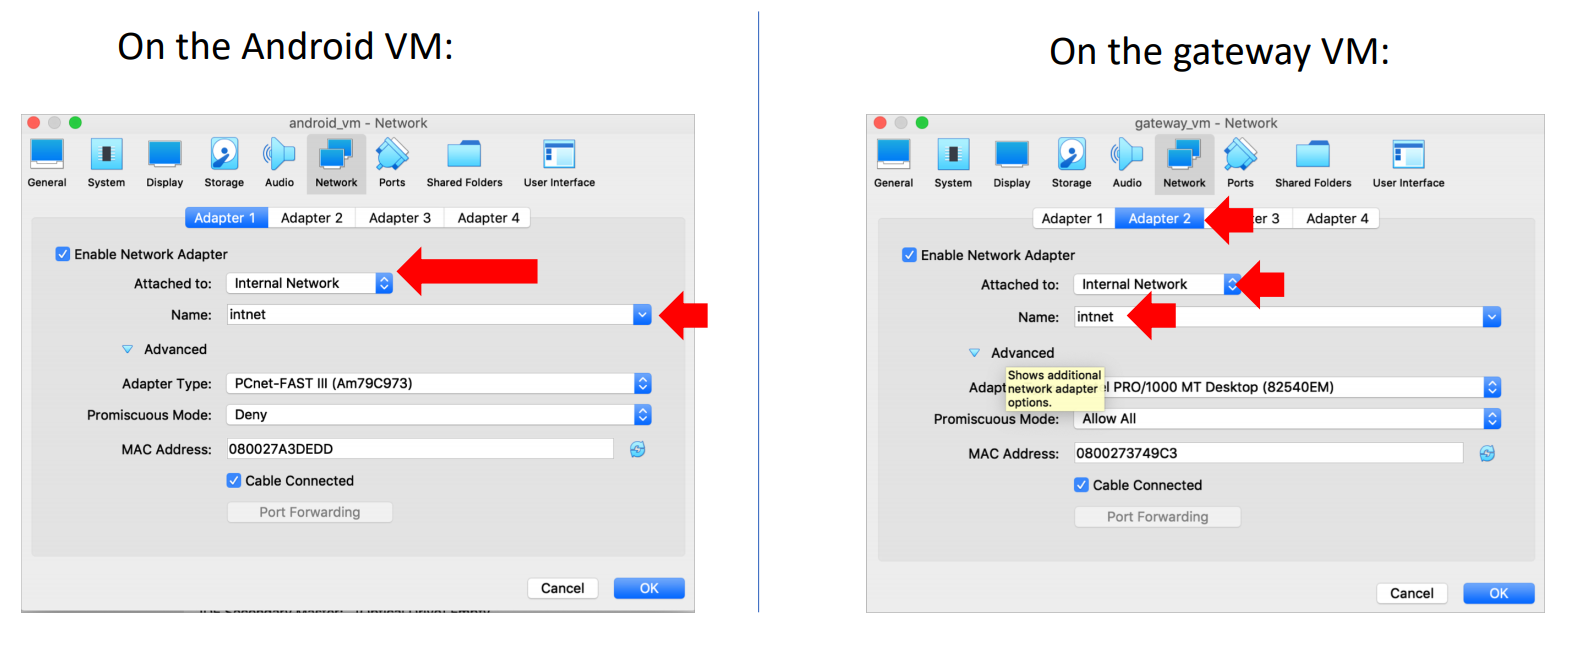
\includegraphics[width=\textwidth]{virtualbox-config.png}
	\caption{VirtualBox network configuration}
\end{figure}

\subsubsection{Startup Script}

Finally, we needed to persist these changes so they apply every time the
TinyCore VM reboots. We wrote this script, \texttt{/opt/eth1.sh}, to run at
startup and apply all the configurations. This script kills the udhcpc process
if it's already running, configures eth1 interface, and then starts the udhcpc
server process.

\begin{lstlisting}[language=bash]
#! /bin/sh

# kill dhcp client for eth1
if [ -f /var/run/udhcpc.eth1.pid ]; then
    kill `cat /var/run/udhcpc.eth1.pid`
    sleep 0.1
fi

# configure interface eth1
ifconfig eth1 192.168.12.1 netmask 255.255.255.0 broadcast 192.168.12.255 up

# start the DHCP server process in the background once the interface is ready
sudo udhcpd /etc/eth1_udhcpd.conf &
\end{lstlisting}

\subsection{Phase 2}
\label{phase-2}

For this phase, we wrote a Python script called \texttt{logFlows} that captures
packets from the Android VM and separates them into bursts and flows. A flow is
defined as a sequence of packets with the same source IP, source port,
destination IP, and destination port. A burst is a group of flows separated by
gaps of greater than one second of silence. After each burst, the program prints
a report on which each flow in that burst, in the following format:

\noindent\texttt{<timestamp> <src addr> <dst addr> <src port> <dst port> <proto>}

\noindent\texttt{<\#packets sent> <\#packets rcvd> <\#bytes send> <\#bytes rcvd>}

As our program is capturing packets, we record each ``half'' flow, which is the
traffic going in a single direction. At the end of a burst, we match each half
flow to its corresponding half flow in order to create a ``full'' flow which
encapsulates all of the traffic going between two hosts.

We have a daemon process that runs in the background in order to detect the end
of a burst during live packet capture. This process checks every fifth of a
second to see if the last packet received is over one second old. If this is the
case, the recorded half flows are matched into full flows and the statistics for
each flow are printed to the standard output.

\subsection{Phase 3}

In Phase 3, we implemented an offline machine learning classifier. We wrote a
script, \texttt{pcapper.py}, that runs on the TinyCore gateway VM, captures
packets from eth1, and writes them to PCAP files. Another script,
\texttt{trainer.py}, builds a classification model based on the feature vectors
described below (see Section~\ref{classification-vectors}). The final script,
\texttt{classifyFlows}, takes in a PCAP packet trace and the model created by
\texttt{trainer.py}, and attempts to identify which application each flow in the
PCAP file came from.

\subsubsection{Classification Vectors}
\label{classification-vectors}

While we were in the process of trying to make the machine learning component as
accurate as possible, we continually added features in the hopes of improving
the accuracy of the model. Our feature vector originally contained only five
elements, and expanded to fourteen elements as we iterated on our strategy for
machine learning.

The following elements within the feature vector are as follows:

\begin{itemize}
    \item Byte ratio (bytes sent / bytes received, or reciprocal)
    \item Packet ratio (packets sent / packets received, or reciprocal)
    \item Mean packet length
    \item Standard deviation of packet lengths (zero if $n \leq 2$)
    \item Packet length kurtosis
    \item Packet length skew
    \item Mean time gap between each packet (zero if $n \leq 1$)
    \item Time gap kurtosis
    \item Time gap skew
    \item Min packet length
    \item Max packet length
    \item Min time gap
    \item Max time gap
    \item Protocol (1 for TCP, 0 for UDP)
\end{itemize}

As you can see from the list above, the bulk of the features are statistical
measure for two main lists. The first list is simply the lengths of all of the
packets in the flow. The second list is the gaps of time between each packet
arrival. Because this list records the intervals, if there were only two packets
in a flow, this list is only one item long.

\subsubsection{Test Data}

We collected four rounds of packet traces for each of the applications being
tested.  Each round of training data collection took around thirty minutes to an
hour. Certain applications generated many megabytes of data. This was especially
true for applications that regularly streamed video, such as YouTube. Other
applications generated far less traffic, such as Fruit Ninja, which played ads
at relatively infrequent intervals. In total, we collected 314 MiB of data in
order to train our classifier.

\subsubsection{Classification Model}

Our first attempt at a classification model used support vector
classification. The implementation of this classifier in sklearn currently has
issues with data containing very large and very small numbers; the classifier
took many minutes to train instead of seconds. Because of this, it was difficult
to work with as we rapidly collected more data to train our model. We tried to
do our own normalization, but this did not help appreciably.

Because of these difficulties, we moved to a random forest classifer. We were
able to train this model much more quickly than our previous method, and this
model appeared to provide better accuracy.

\begin{table}[h]
	\centering
	\begin{tabular}{l r r}
		Application Name & \% Correct & \% Unknown \\
		\hline
		YouTube & 79.94\% & 11.39\% \\
		Browser & 20.53\% & 34.48\% \\
		Google News & 36.13\% & 24.44\% \\
		Fruit Ninja & 53.33\% & 11.76\% \\
		Weather Channel & 55.84\% & 20.10\% \\
		\textbf{Average} & \textbf{50.15\%} & \textbf{20.43\%} \\
	\end{tabular}
	\caption{Phase 3 accuracy}
\end{table}

Excluding unknown flows we were able to get above 50\% accuracy. Additionally,
each application's accuracy was better than simply guessing ($> 20\%$).

\subsection{Phase 4}

For this phase we combined all the previous phases to make a complete project.
Since we trained the model on a 64-bit machine for Phase 3, we had to retrain
the model to work on 32-bit TinyCore. We then set it up to run continuously on
the VM. It captures live packets from the Android VM and classifies them in real
time, writing the results of each classification to standard output.

The Python script that performs this live classification is called
\texttt{analyzeFlows}. This is essentially a modified version of
\texttt{classifyFlows} from Phase 3 that sniffs packets and performs
classification in real time instead of from a PCAP file. At the end of a burst,
each flow is printed in the format specified in Section~\ref{phase-2}, but also
prints out the predicted application name for each flow. If the classifier is
not particularly confident about any one classification, ``unknown'' is printed
in place of the application name.

\section{Lessons Learned and Limitations}

The first machine learning-related hurdle was our difficulty getting the model
trained in a reasonable amount of time. We tried to use a support vector
classifier in both linear and polynomial modes. Neither had good performance,
and they both took a very long time to train, even with small amounts of data
and very short feature vectors. We discovered that this was an inherent problem
with sklearn's implementation of this classifier, which has issues with data
that is not normalized. The random forest classifier did not have these issues,
so we elected to retrain our model with this classifier partway through Phase 3
of the project.

The other issue that prevented us from attaining a higher accuracy was that the
process of collecting training data was quite slow. We could have elected to
automate this process, but we were hesitant to do so because we were concerned
this would bias the classifier with data produced by non-human interaction with
the software.

We also had some trouble with configuring TinyCore in Phase 1 since it is very
different from most GNU/Linux installations. We fixed these issues by
essentially starting over from scratch.

Our choice of classification model and design of feature vectors were not
entirely educated because neither of us have taken a machine learning class. We
also had no experience with scikit-learn. We tried to educate ourselves on how
these models worked, but despite our efforts they essentially remained a ``black
box'' due to the time constraints.

We were puzzled as to why our classifier was strongly biased towards the Weather
Channel app. We hypothesize that the Weather Channel's app performs a variety of
network applications including video, advertisements, and asynchronous data
requests, which makes it easy to confuse with other apps. Perhaps a more
thorough understanding of how classifiers work would have helped us understand
this issue better.

Although our classifier was not perfect, it exceeded our expectations by being
right most of the time, when excluding unknown flows.

\end{document}
